\chapter{Métodos estatísticos e simbólicos aplicados na análise de sentimentos}
\label{cap:Classificadores}

Antigamente, para sabermos a opinião de outras pessoas sobre um
determinado produto, tinhamos que perguntar diretamente a essas pessoas. Com a
popularização da Internet e também de redes sociais, milhares de pessoas
compartilham as suas opinões sobre produtos, política, serviços e
demais assuntos. Porém, muitas vezes essas opiniões acabam
por ser esquecidas devido a dificuldade em analisar uma grande quantidade de
textos. De fato, uma das maiores dificuldades reside em como obter a opinião
geral das pessoas sobre determinado produto em uma seção de comentários com mais
de 1000 opiniões diferentes. Dentro dessa contexto, a análise de sentimentos,
tem como função identificar e quantificar os sentimentos expressos através de
textos.

Neste capítulo serão descritos um método estatístico (\textit{Naive Bayes}) e um
método simbólico (\ac{VADER}), que podem ser aplicados na análise de sentimentos.
Outros possíveis métodos estatísticos para a análise de sentimentos são \ac{SVM}
\cite{Hearst:1998:SVM:630302.630387} e \ac{MaxEnt}
\cite{Berger:1996:MEA:234285.234289}, os quais possuem performance similar ao Naive Bayes \cite{Pang:2002:TUS:1118693.1118704}. Ambos métodos serão descritos para o uso da língua Inglesa, visto que o \textit{Website} analisado (Reddit) possui a maioria de seus
comentários em língua Inglesa. Além disso, não foram encontrados métodos que
façam uso da língua Portuguesa com similar precisão.




%Para o \ac{NLP} e também para o campo de estatísticas, classificadores são
%algorítmos que identificam a qual categoria determinado item pertence. Essa
%classificação é feita a partir de dados já classificados corretamente, ou seja,
%um \textit{training set}.

\section{Método de Naive Bayes}

O Naive Bayes é um método estatístico para a classificação e que pode ser
utilizado para a análise de sentimento. Esse faz o uso do teorema de Bayes e um
\textit{training set} para inferir a classificação de uma frase. Por exemplo,
considerando que se quer determinar se a frase \textit{``This place is
great''} demonstra um sentimento negativo ou positivo.

\begin{table}[htb]
\centering
\begin{tabular}{|l|l|}
\hline
Texto  & Categoria \\ \hline
The food was great  & Positiva     \\ \hline
They are horrible!    & Negativa     \\ \hline
I love the food here  & Positiva     \\ \hline
This place is wonderful  & Positiva     \\ \hline
Forgettable experience  & Negativa     \\ \hline
\end{tabular}
\caption{\textit{Training Set}}
\label{tab:trainingsetnb}
\end{table}

A partir do \textit{training set} hipotético (Tabela
\ref{tab:trainingsetnb}) será calculada a probabilidade da frase
\textit{``This place is great''} ser positiva e também de ser negativa sendo que
a partir dessas duas possibilidades, será escolhida a de maior probabilidade.

Para cálcular a probabilidade da frase \textit{``This place is great''}
pertencer a cada categoria é utilizado o teorema de Bayes \cite{manningschutze1999}, através da Equação
\ref{eq:teorema}. Na Equação \ref{eq:teorema}, o termo P(c$\vert$d) corresponde
a probabilidade da frase \textbf{d} pertencer a classe \textbf{c}, ou seja, a
probabilidade de \textit{``This place is great''} ser uma frase positiva ou negativa. O Termo P(d$\vert$c) é a probabilidade da
  classe \textbf{c} ser a frase \textbf{d}, ou seja, dentre todas as frases
  negativas ou positivas, a probabilidade de uma das frases ser \textit{``This
  place is great''}. Já P(c) é a probabilidade de frases negativas ou positivas
  aparecerem em nosso \textit{training set}. E, por fim, P(d) é a probabilidade
  da frase \textit{``This place is great''} aparecer em nosso \textit{training
  set}.

\begin{equation}
\begin{gathered}
P(c|d) = \frac{P(d|c) \times P(c)}{P(d)} \\
\label{eq:teorema}
\end{gathered}
\end{equation}

\begin{equation}
\begin{gathered}
P(Negativa|\textit{This place is great})
=
\frac{P(\textit{This place is great}|Negativa) \times
P(Negativa)}{\textit{This place is great}}
\label{eq:teoreman1}
\end{gathered}
\end{equation}
\begin{equation}
\begin{gathered}
P(Positiva|\textit{This place is great})
=
\frac{P(\textit{This place is great}|Positiva) \times
P(Positiva)}{\textit{This place is great}}
\label{eq:teoremap1}
\end{gathered}
\end{equation}


Uma vez que as Equações \ref{eq:teoreman1} e \ref{eq:teoremap1}
apresentam P(d) como divisor (\textit{``This place is great''}), essas podem ser
simplificadas resultando nas Equações \ref{eq:teoreman} e \ref{eq:teoremap}.
\begin{equation}
\begin{gathered}
P(Negativa|\textit{This place is great})
=
P(\textit{This place is great}|Negativa) \times
P(Negativa)
\label{eq:teoreman}
\end{gathered}
\end{equation}
\begin{equation}
\begin{gathered}
P(Positiva|\textit{This place is great})
=
P(\textit{This place is great}|Positiva) \times
P(Positiva)
\label{eq:teoremap}
\end{gathered}
\end{equation}



Nas Equações \ref{eq:teoreman} e \ref{eq:teoremap}, os termos P(Positiva) e
P(Negativa) são definidos pela frequência que frases positivas e negativas aparecem no \textit{training set}, sendo determinados
através das Equações \ref{eq:frasespositivas} e \ref{eq:frasesnegativas}. Como
pode ser observado, os valores de P(positiva) e P(negativa) correspondem a 0,6
e 0,4 respectivamente, uma vez que em nosso \textit{training set} tem-se um
total de 5 frases onde 3 dessas são positivas (Equação \ref{eq:frasespositivas})
e as outras 2 são negativas (Equação \ref{eq:frasesnegativas}).

\begin{equation}
\begin{gathered}
P(Positiva)
=
\frac{3}{5} = 0,6
\label{eq:frasespositivas}
\end{gathered}
\end{equation}
\begin{equation}
\begin{gathered}
P(Negativa)
=
\frac{2}{5} = 0,4
\label{eq:frasesnegativas}
\end{gathered}
\end{equation}

Uma vez que a frase \textit{``This place is great''} não existe por completo no
\textit{training set}, tem-se que o termo P(d$\vert$c) da Equação
\ref{eq:teoreman} e \ref{eq:teoremap} é igual a zero (0), impossibilitando o
cálculo de probabilidade para essa frase. Neste caso, se faz o uso do
\textit{Naive Bayes}, o qual passa a considerar todas as palavras ao invés da
frase completa. O uso do Naive Bayes elimina o problema de frases que não se
encontram no \textit{training set}. Neste caso, é considerado somente a
frequência que cada palavra aparece em uma frase positiva e em uma negativa.
Portanto, o termo $P(\textit{This place is
great}|Positiva)$ da Equação \ref{eq:teoremap} é dado pela Equação
\ref{eq:frasespositivas1}.

\begin{equation}
\begin{gathered}
P(\textit{This place is great}|Positiva) = P(\textit{This}|Positiva)
\times P(\textit{place}|Positiva) \\ \times P(\textit{is}|Positiva) \times
P(\textit{great}|Positiva)
\label{eq:frasespositivas1}
\end{gathered}
\end{equation}

A partir da Equação \ref{eq:frasespositivas1} é necessário calcular os
termos P(\textit{This}$\vert$Positiva),
P(\textit{place}$\vert$Positiva), P(\textit{is}$\vert$Positiva), P(\textit{great}$\vert$Positiva).
O termo P(\textit{This}$\vert$Positiva) é calculado pela razão entre a
quantidade de vezes que a palavra \textit{This} encontra-se em uma frase
classificada como positiva no \textit{training set}, e o total de palavras que
se encontram em frases classificadas como positiva (Equação
\ref{eq:thispositiva}).

\begin{equation}
\begin{gathered}
P(\textit{This}|Positiva) = \frac{1}{13}
\label{eq:thispositiva}
\end{gathered}
\end{equation}


Da mesma forma, a Equação \ref{eq:thispositiva} deve ser aplicada para as demais
palavras da frase \textit{``This place is great''}, obtendo-se os valores
apresentados na Tabela \ref{tab:probabilidadesnb}.

\begin{table}[htb]
\centering
\renewcommand{\arraystretch}{1.5}% Spread rows out...
\begin{tabular}{lll}
\hline

Palavra & Positiva & Negativa \\ \hline
This & \large $\frac{1}{13}$ & \large $\frac{0}{5}$ \\
place & \large $\frac{1}{13}$ & \large $\frac{0}{5}$ \\
is & \large $\frac{1}{13}$ & \large $\frac{0}{5}$ \\
great & \large $\frac{1}{13}$ & \large $\frac{0}{5}$ \\
\end{tabular}
\caption{Tabela de Palavras e Probabilidades.}
\label{tab:probabilidadesnb}
\end{table}

Uma vez que algumas palavras não encontram-se no \textit{training set}
essas acabam zerando o resultado final da
multiplicação das probabilidades (Equação
\ref{eq:frasespositivas1}). De modo, a evitar que uma única palavra
invalide a frase por completo é utilizado o método \textit{Laplace smoothing}
\cite{Manning:2008:IIR:1394399}. Neste, é somado 1 a cada palavra da frase. Já
ao total de palavras positivas é somada a quantidade de palavras distintas do
\textit{training set} (16). Aplicando o \textit{Laplace smoothing} para os
valores apresentados na Tabela \ref{tab:probabilidadesnb} são obtidos os valores
que se encontram na Tabela \ref{tab:probabilidadesl}.


\begin{table}[htb]
\centering
\renewcommand{\arraystretch}{1.5}% Spread rows out...
\begin{tabular}{lll}
\hline

Palavra & Positiva & Negativa \\ \hline
This & \large $\frac{1 + 1}{13 + 16}$ & \large $\frac{0 + 1}{5 + 16}$ \\
place & \large $\frac{1 + 1}{13 + 16}$ & \large $\frac{0 + 1}{5 + 16}$ \\
is & \large $\frac{1 + 1}{13 + 16}$ & \large $\frac{0 + 1}{5 + 16}$ \\
great & \large $\frac{1 + 1}{13 + 16}$ & \large $\frac{0 + 1}{5 + 16}$ \\
\end{tabular}
\caption{Tabela de Probabilidades - \textit{Laplace smoothing}.}
\label{tab:probabilidadesl}
\end{table}

Utilizando as probabilidades que são apresentadas na Tabela
\ref{tab:probabilidadesl} na Equação \ref{eq:frasespositivas1} tem-se:

\begin{equation}
\begin{gathered}
P(Positiva|\textit{This place is great}) = \frac{1 + 1}{13 + 16} \times
\frac{1 + 1}{13 + 16} \times \frac{1 + 1}{13 + 16} \times
\frac{1 + 1}{13 + 16} = 0,000023.
\label{eq:ppositivaplace}
\end{gathered}
\end{equation}

Uma vez que o termo P(Positiva $\vert$ \textit{This place is great})
encontra-se definido, esse pode ser utilizado na Equação \ref{eq:teoreman},
onde o termo P(Positiva) é igual a 0,6 (Equação \ref{eq:frasespositivas}). Neste caso, tem-se que a probabilidade da
frase \textit{``This place is great''} ser classificada como positiva é

\begin{equation}
\begin{gathered}
P(Positiva|\textit{This place is great})
=
0,000023 \times
0,6 = 0,0000138.
\label{eq:positiva}
\end{gathered}
\end{equation}

Efetuando o mesmo processo para a probabilidade da frase ser negativa, tem-se:
\begin{equation}
\begin{gathered}
P(Negativa|\textit{This place is great})
=
0,0000049 \times
0,4 = 0,00000196.
\label{eq:negativa}
\end{gathered}
\end{equation}

Portanto, tem-se que a frase ``This place is great'' é positiva, uma vez que a
probabilidade de ser positiva (0,0000138) é maior que a probabilidade dessa
frase ser negativa (0,00000196).

\section{Método de \textit{VADER}}

O método de \ac{VADER} é um dicionário e classificador de sentimentos que se
baseia em regras, portanto, um método de classificação simbólico. Esse foi desenvolvido
especificamente para ser utilizado em redes sociais, onde se tem um contexto
vago, pouca quantidade de texto, gírias e \textit{emoticons}
\cite{conf/icwsm/HuttoG14}.

A classificação do sentimento é feita através da separação da frase em palavras,
sendo que para cada palavra da frase é atribuída uma pontuação de intensidade em
uma escala de -4 (sentimento negativo) até +4 (sentimento positivo). Como por
exemplo, a palavra \textit{great} tem a intensidade de 3.1 e \textit{horrible} -2.5. Essa pontuação é obtida através de
um dicionário que é construído utilizando o método de \textit{``wisdom of the
crowd''}, onde um grupo de pessoas é responsável por atribuir os valores de
intensidade para cada palavra. Por exemplo, a frase \textit{``This place is great''} seria classificada com


\begin{table}[htb]
\centering
\begin{tabular}{l|l|l|l|l|l|l}
Palavra         & \textit{This}        & \textit{place} & \textit{is}      &
\textit{great}
\\
%Correta: & Substantivo & Verbo  & Artigo & Substantivo & Preposição &
% Substantivo \\
Intensidade:   &  &   &  & 3,1
\end{tabular}
\label{my-label}
\end{table}

As palavras \textit{``This''}, \textit{``place''} e \textit{``is''} são
desconsideradas uma vez que não existem no dicionário e não expressam
sentimentos. Após, essa fase inicial, utiliza-se o seguinte conjunto de regras,
os quais utilizam valores empiricamente derivados para inferir a intensidade
do sentimento \cite{conf/icwsm/HuttoG14}:
\begin{itemize}
\item É verificado quando uma palavra que expressa sentimentos é escrita em letras
maiúsculas.
  Neste caso, é aumentada a magnitude da intensidade do sentimento sem modificar
  a orientação semântica. Isso é feito somando 0,733 na intensidade do
  sentimento caso este tenha intensidade positiva ou subtraindo
  0,733 caso este tenha uma intensidade negativa.
  \begin{table}[htb]
	\centering
	\begin{tabular}{l|l|l|l|l|l|l}
	Palavra         & \textit{This}        & \textit{place} & \textit{is}      &
	\textit{GREAT}
	\\
	%Correta: & Substantivo & Verbo  & Artigo & Substantivo & Preposição &
	% Substantivo \\
	Intensidade:   &  &   &  & 3,1 \textrightarrow 3,833
	\end{tabular}
	\label{my-label}
   \end{table}

\item É verificado se alguma das três palavras anteriores é um advérbio
intensificador. Neste caso, a intensidade do sentimento é aumentada ou diminuida
em 0,293.

  \begin{table}[htb]
	\centering
	\begin{tabular}{l|l|l|l|l|l|l}
	Palavra         & \textit{This}        & \textit{place} & \textit{is}      &
	\textit{incredibly} & \textit{great}
	\\
	%Correta: & Substantivo & Verbo  & Artigo & Substantivo & Preposição &
	% Substantivo \\
	Intensidade:   &  &   &  & Advérbio & 3,1 \textrightarrow 3,393 
	
	\end{tabular}
	\label{my-label}
   \end{table}
   
   
  \begin{table}[!htb]
	\centering
	\begin{tabular}{l|l|l|l|l|l|l}
	Palavra         & \textit{This}        & \textit{place} & \textit{is}      &
	\textit{somewhat} & \textit{great}
	\\
	%Correta: & Substantivo & Verbo  & Artigo & Substantivo & Preposição &
	% Substantivo \\
	Intensidade:   &  &   &  & Advérbio & 3,1 \textrightarrow 2,807
	\end{tabular}
	\label{my-label}
   \end{table}
   

\item É verificado se a frase contém a palavra \textit{``but''}. Essa palavra
indica uma troca do sentimento da frase, uma vez que o texto seguinte a palavra
\textit{``but''} expressa um sentimento dominante. Neste caso, o método
multiplica a intensidade dos sentimentos expressos até a palavra
\textit{``but''} por 0,5 e os sentimentos expressos após a palavra
\textit{``but''} por 1,5.

   
   \begin{table}[!htbp]
	\centering
	\begin{tabular}{l|l|l|l|l|l|l|l|l}
	Palavra         & \textit{Great} & \textit{place}      & \textbf{\textit{but}}
	& \textit{today} & \textit{the}      &
	\textit{food} & \textit{was}      & \textit{horrible}
	\\
	%Correta: & Substantivo & Verbo  & Artigo & Substantivo & Preposição &
	% Substantivo \\
	Intensidade: & 3,1 \textrightarrow 1,55  &   &  &  & & & &  -2,5
	\textrightarrow -3,75
	\end{tabular}
	\label{my-label5}
   \end{table}

\item É verificado se a frase possui pontos de exclamação (!). Este
tipo de pontuação aumenta a magnitude da intensidade sem modificar a
orientação semântica. Neste caso, é adicionado um valor de 0,292 a cada
ponto de exclamação, considerando um máximo de 4 pontos de exclamação.

 \begin{table}[!htbp]
	\centering
	\begin{tabular}{l|l|l|l|l|l|l}
	Palavra         & \textit{This}        & \textit{place} & \textit{is}      &
	\textit{great!}
	\\
	%Correta: & Substantivo & Verbo  & Artigo & Substantivo & Preposição &
	% Substantivo \\
	Intensidade:   &  &   &  & 3,1 \textrightarrow 3,392
	\end{tabular}
	\label{my-label}
   \end{table}
   

\item São examinadas as três palavras anteriores,
procurando a existência de uma negação que inverta a polaridade do texto.
Quando é encontrada uma negação na frase, a intensidade de cada palavra de
sentimento é multiplicada por -0,74.

 \begin{table}[!htbp]
	\centering
	\begin{tabular}{l|l|l|l|l|l|l}
	Palavra         & \textit{This}        & \textit{place} & \textit{wasn't}     
	&
	\textit{great}
	\\
	%Correta: & Substantivo & Verbo  & Artigo & Substantivo & Preposição &
	% Substantivo \\
	Intensidade:   &  &   & Negação & 3,1 \textrightarrow -2,294
	\end{tabular}
	\label{my-label}
   \end{table}


\end{itemize}

Após o cálculo de intensidade, é feita a normalização dessa
pontuação, a partir da Equação \ref{eq:vader}. Neste caso, 15 é um valor
fixo para aproximar o resultado final do valor máximo esperado (-1 para
palavras negativas e +1 para palavras positivas).

\begin{equation}
\begin{gathered}
\text{Pontuação Normalizada}
=
\frac{\text{Pontuação}}{\sqrt{\text{Pontuação}^2 + 15}}
\label{eq:vader}
\end{gathered}
\end{equation}


\begin{equation}
\begin{gathered}
\text{Pontuação Normalizada}
=
\frac{\text{3,1}}{\sqrt{\text{3,1}^2 + 15}} = 0,6249
\label{eq:vaderscore}
\end{gathered}
\end{equation}

Neste caso para a frase \textit{``This place is great''}, será
atribuída uma pontuação final de 0,6249.  Caso a
pontuação da frase fosse menor que -1 ou maior que 1, essa seria limitada aos
valores de -1 ou 1, respectivamente. Para o \ac{VADER}, são consideradas frases negativas
aquelas que apresentam uma pontuação de -1 até -0,5, frases neutras aquelas que
apresentam uma pontuação de -0,5 até 0,5 e frases positivas aquelas que
apresentam uma pontuação 0,5 até 1.
Portanto, a frase \textit{``This place is great''} com pontuação de 0,6249 seria
classificada como positiva.

\subsection{Definição de Método para Identificação de Sentimentos}

Para o desenvolvimento deste trabalho optou-se pelo uso do método de \ac{VADER},
uma vez que este, segundo a literatura, apresenta resultados superiores ao
Método de Naive Bayes. De fato, segundo Pålsson e Szerszen
\cite{SentimentinSocialMedia}, para a análise de
\textit{tweets}\footnote{\textit{Tweets} é o termo utilizado para designar as publicações realizadas na rede social Twitter.}, o método de
\ac{VADER} apresentou uma assertividade de 72,3\% enquanto o Naive Bayes apresentou uma assertividade de apenas 58,2\%.

Na análise conduzida por Hutto \cite{conf/icwsm/HuttoG14},
considerando-se a análise de \textit{tweets}, avaliações de produtos da Amazon e
editoriais do New York Times, o método de \ac{VADER} apresentou uma assertividade de 96\%, 63\% e 55\%, respectivamente, contra
56\%, 49\%, 44\% do método de Naive Bayes. A Figura \ref{fig:definicao}
apresenta um resumo dos resultados demonstrados na literatura.

\begin{figure}[htbp] 

 \begin{framed}\raggedleft%\centering
 \centering 
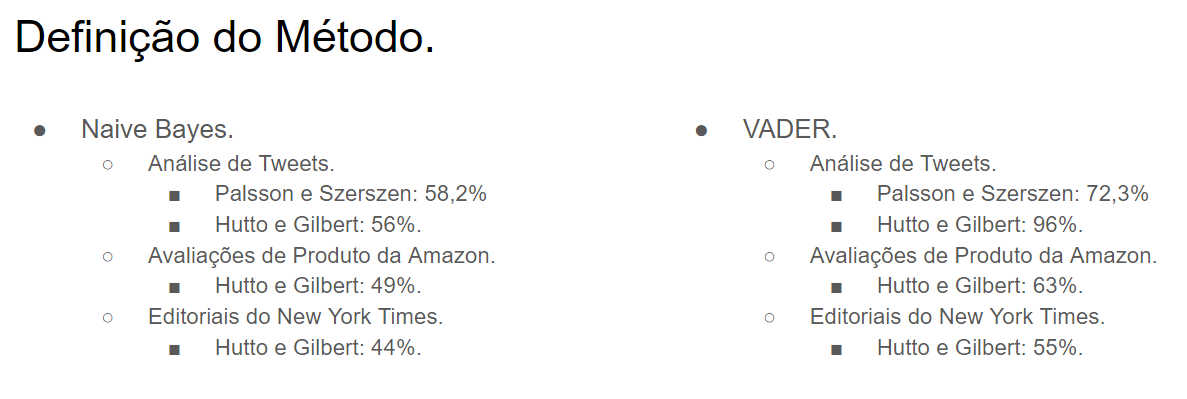
\includegraphics[height=120px]{imagens/definicao.png}
\end{framed}
\caption{Resultados obtidos para definição do método.}
\label{fig:definicao}
\end{figure}

Destaca-se ainda que o método de \ac{VADER} possui uma maior
adaptabilidade, uma vez que esse não necessita do desenvolvimento de um
\textit{training set} específico para o tema que está sendo analisado.
Desta forma, sendo o mais adequado para a análise de sentimentos na rede social
Reddit, visto que os tópicos que foram selecionados neste trabalho abrangem uma
quantidade diversificada de assuntos, o que inviabiliza a especialização de um
\textit{training set} para cada um dos tópicos.


\subsection{NLTK - \textit{Natural Language Toolkit}}

A implementação de um software de análise de sentimentos pode ser feita através
do desenvolvimento de um \textit{software} por completo, ou através da
utilização de \textit{frameworks} já disponíveis.
Métodos estatísticos, como o Naive Bayes, podem ser encontrados tanto em
\textit{frameworks} de aprendizado de máquina, quanto em \textit{frameworks}
voltados para o \ac{NLP}.
Já os métodos simbólicos, por suas implementações serem específicas para o
\ac{NLP} ou análise de sentimentos, somente são encontrados em
\textit{frameworks} de \ac{NLP}.

O método de \ac{VADER}, que será utilizado nesse trabalho, encontra-se
disponível como um \textit{package} Python \cite{Rossum:1995:PRM:869369}, ou
ainda, através do \textit{framework} \ac{NLTK}
\cite{Loper:2002:NNL:1118108.1118117}, o qual implementa diversos métodos de
\ac{NLP}, incluindo métodos para análise de sentimentos. Neste trabalho,
optou-se pelo uso do \textit{framework} \ac{NLTK}, devido a possibilidade de uma
futura de utilização de outros métodos de \ac{NLP} para a análise de
sentimentos.

O \ac{NLTK} é um \textit{framework open source} para Python que foi
criado em 2001 na Universidade de Pensilvânia e, atualmente, é utilizado por
mais de 30 universidades em diversos
países \cite{nltk}.
Esse apresenta tanto métodos estatísticos como, \ac{MaxEnt} e Naive Bayes, como
métodos simbólicos, contendo mais de 50 dicionários e modelos já treinados.
Além do \ac{VADER}, pode-se citar o conjunto de dados \textit{Sentiment
Polarity Dataset Version 2.0}, que contém mais de 1000 filmes classificados de
forma positiva e 1000 filmes classificados de forma negativa
\cite{Pang:2002:TUS:1118693.1118704}.
Além disso, destaca-se o \textit{SentiWordNet} que é um dicionário com as
palavras extraídas do WordNet já classificadas em positividade, negatividade e objetividade \cite{Esuli2006sentiwordnet}.

